\title{Implementing Ray-Tracing Algorithm}
\author{qiangzhiwen 515030910367}
\date{}
\documentclass{article} 
\usepackage{graphicx}
\usepackage{xcolor}
\usepackage{listings}
 \usepackage{mathrsfs}
 \usepackage{amsfonts,amssymb}
 
\begin{document} 
\maketitle{}
\section{Question}
Write a program to implement the ray tracing or ray casting algorithm to synthesis an image of some virtual environment (with some graphical objects of your own choice). The image should contain the show effect of the virtual environment.

\section{Principle}
\begin{itemize}
\item Deciding the primary ray of the scene.
\item Check every object of the scene to see if it intersects with the ray.
\item If no, this point is illuminated, otherwise, that object cast a shadow on it.
\item Incorporating computations for both reflection and  refraction.
\end{itemize}

\section{My Work}
\begin{itemize}
\item Create Point Class in three dimension, overload its basic operation
\item Create Sphere Class using the Point Class, create the properties including position, radius, surface color, reflectivity, transparency and emission color.
\item Construct the trace function, which takes a ray as argument then test if this ray intersects any of the geometry in the scene. If does, compute the intersection point, then normalize at the intersection point, and shade this point depending on the surface property (transparent, reflective, diffuse). Otherwise it returns
the background color.
\item Construct the render function, which compute a camera ray for each pixel, then trace it and return a color. Return the color of the sphere at the intersection point if the ray hits a sphere, otherwise return the background color.
\item Construct the main function, which create the scene composed of 6 spheres and 1 light. Then, we call the render function once the scene is ready.

\end{itemize}
\section{How to run}
I run this program on Ubuntu 14.04 environment.
You could use IDE like codeblocks to build this program, after compiling, open the $raytracing.ppm$ file and you will see the results.

\section{Output}
\begin{figure}[htbp]
	\centering
	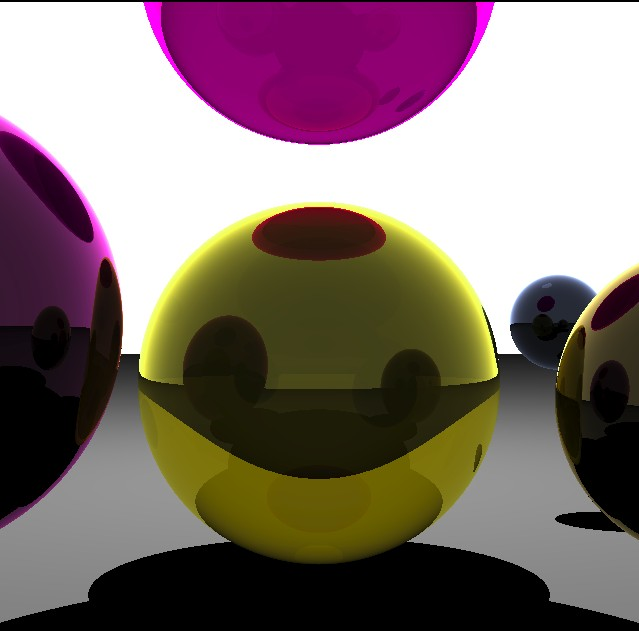
\includegraphics[width=12cm]{raytracing.jpg}
\caption{Result of ray tracing}

\end{figure}


\end{document} 